\documentclass{article}

% Langue
\usepackage[utf8]{inputenc}
\usepackage[T1]{fontenc}      
\usepackage[francais]{babel}

% Mise en forme générale
\usepackage[top=2.5cm,bottom=2.5cm,right=2.5cm,left=2.5cm]{geometry}

% Package divers
\usepackage{chemist} 
\usepackage[version=3]{mhchem}
\usepackage{chemfig}
\usepackage[squaren, Gray]{SIunits}
\usepackage{sistyle}
\usepackage[autolanguage]{numprint}
\usepackage{url}
\usepackage{rotating}
\usepackage{xcolor,colortbl}
\definecolor{Gray}{gray}{0.85}

\usepackage{hyperref}
\hypersetup{
    colorlinks,
    citecolor=black,
    filecolor=black,
    linkcolor=black,
    urlcolor=black
}

% Nouvelles commandes
\newcommand{\std}{\ensuremath{^{\circ}}}
\newcommand\ph{\ensuremath{\mathrm{pH}}}
\newcommand{\annexe}{\part{Annexes}\appendix}
\newcommand{\biblio}[1]{\bibliographystyle{plain}\bibliography{#1}\nocite{*}}

\newcommand{\doctitle}[1]{
	\title{#1}
	\author{\textbf{Groupe 124.3}\\
	\textsc{Frenyo} Péter (6266-12-00)\\
	\textsc{Gillain} Nathan (7879-12-00)\\
	\textsc{Lamine} Guillaume (7109-13-00)\\
	\textsc{Piraux} Pauline (2520-13-00)\\
	\textsc{Paris} Antoine (3158-13-00)\\
	\textsc{Quiriny} Simon (4235-13-00)\\
	\textsc{Schrurs} Sébastien (7978-13-00)}
	\date{\today}

	\begin{document}

	\maketitle
	\tableofcontents
}

\doctitle{Projet 3 - Synthèse}
\newpage
\section{Thermochimie}
\subsection{Notion d'équilibre réactionnel}
Soit une réaction chimique quelconque
\begin{chemmath}
	lL + mM  \Leftrightarrow xX + yY.
\end{chemmath}
Pour cette réaction, on peut écrire un
degré d'avancement $\xi(t)$ défini comme
suit
\[ \xi(t) = \frac{n_X(t) - n_{X0}}{x} =
\frac{n_Y(t) - n_{Y0}}{y} = \frac{n_L0 - n_{L}(t)}{l}
= \frac{n_M0 - n_{M}(t)}{m}. \]
Une réaction est spontanée si sa variation
d'enthalpie libre est négative 
\[ \frac{\mathrm{d}G}{\mathrm{d}\xi}(\xi) < 0. \]
A l'équilibre on aura 
\[ \frac{\mathrm{d}G}{\mathrm{d}\xi}(\xi_{eq}) = 0.\]
Or, on sait (cfr. cours de thermodynamique de première) que
\[ \frac{\mathrm{d}G}{\mathrm{d}\xi} = \Delta G^{\circ}(T)
+ RT\ln{Q_r(\xi,p,T)}\]
où $Q_r(\xi,p,T)$, le quotient réactionnel, est
défini en fonction des activités des composés
\[ Q_r(\xi,p,T) = \frac{(a_X(\xi))^x(a_Y(\xi))^y}{(a_L(\xi))^l(a_M(\xi))^m}. \]
Pour rappel, les activités dépendant de la phase
de l'élement :
\begin{itemize}
	\item Solides et liquides pures : $a=1$ ;
	\item Gaz : $a = \frac{p}{p^{\circ}}$ avec
	$p^{\circ} = \unit{1}{\bbar}$ la pression standard ;
	\item Solutions aqueuses : $a = \frac{c}{c^{\circ}}$
	avec $c^{\circ} = \unit{1}{\mole\per\liter}$ la concentration
	standard.
\end{itemize}
On définit enfin la constante d'équilibre 
\[ K(t) = Q_r(\xi_{eq}) = \exp{-\frac{\Delta G^{\circ}(T)}{RT}}. \]

\subsection{Notion d'enthalpie de réaction}
Pour la même réaction quelconque que dans la section
précédente, on définit l'enthalpie de réaction
\[ \Delta H\std = x\Delta H\std_{form,X} + y\Delta H\std_{form,Y}
- l\Delta H\std_{form,Y} - m\Delta H\std_{form,M}.\]
Cette enthalpie, qui correspond à la chaleur de réaction 
est souvent exprimée en \unit{}{\joule\per\kilo\gram}
ou en \unit{}{\joule\per\mole} d'un composé présent en quantité
stoéchiométrique égale à 1. Si l'enthalpie de réaction est négative,
alors ça correspond à de la chaleur dégagée par le
système, la réaction est alors exothermique. Si au contraire
elle est positive, ça correspond à de la chaleur absorbée
par le système, la réaction est alors entothermique.

\paragraph{Influence de la température} L'enthalpie
varie avec la température
\[ \Delta H\std(T_2) = \Delta H\std(T_{ref})
+ \int_{T_1}^{T_2} \Delta C_p \mathrm{d}T \]
où $\Delta C_p$ est la différences des capacités
calorifiques molaires des produits et des réactifs
pondérées par leur coefficient stoéchiométrique.
\paragraph{Influence de la pression} L'enthalpie
ne dépend pas de la pression.

TODO : ajouter entropie et enthalpie de libre comme
c'est quand même utilisé dans le projet pour calculer
les constantes d'équilibre.

\subsection{Calcul d'un équilibre global pour plusieurs réactions simultanées
(comme dans le réformeur primaire)}
Dans le réformeur primaire, nous avons dans un premier temps
calculer les constantes d'équilibre $K_1$ et $K_2$ des deux 
réactions à partir de l'enthalpie libre. Nous avons ensuite
dressé deux tableaux d'avancement.

	\begin{table}[ht!]
		\centering
		\begin{tabular}{c|cccccccc}
									& \ce{CH_4(g)} 				&+& \ce{H_2O(g)} 			 	&	$\Leftrightarrow$ 		& \ce{CO(g)} 			&+& \ce{3H_2(g)} \\
			\hline
			$n_i$ 			& $n_{01}$ 						& & $n_{02}$						& 											& 0								&	& 0 \\
			$n_{eq}(x)$	&	$n_{01}-x$ 					& & $n_{02}-x-y$				& 											& $x-y$ 					&	& $3x+y$ \\
			\hline 
			$a_{eq}$		& $\frac{n_{01}-x}{n_{gaz,tot}}\frac{p}{p\std}$ &
																				& $\frac{n_{02}-x-y}{n_{gaz,tot}}\frac{p}{p\std}$ &
																															& $\frac{x-y}{n_{gaz,tot}}\frac{p}{p\std}$ &
																																									& $\frac{3x+y}{n_{gaz,tot}}\frac{p}{p\std}$
		\end{tabular}
		\caption{Tableau d'avancement de la première réaction.}
		\label{avancement1}
	\end{table}
	
	\begin{table}[ht!]
		\centering
		\begin{tabular}{c|cccccccc}
									& \ce{CO(g)} 				&+& \ce{H_2O(g)} 			 		&	$\Leftrightarrow$ 		& \ce{CO_2(g)} 			&+& \ce{H_2(g)} \\
			\hline
			$n_i$ 			& $x$ 							& & $n_{02}-x$						& 											& 0								&	& $3x$ \\
			$n_{eq}(x)$	&	$x-y$ 						& & $n_{02}-x-y$					& 											& $y$ 						&	& $3x+y$ \\
			\hline 
			$a_{eq}$		& $\frac{x-y}{n_{gaz,tot}}\frac{p}{p\std}$ &
																				& $\frac{n_{02}-x-y}{n_{gaz,tot}}\frac{p}{p\std}$ &
																															& $\frac{y}{n_{gaz,tot}}\frac{p}{p\std}$ &
																																									& $\frac{3x+y}{n_{gaz,tot}}\frac{p}{p\std}$
		\end{tabular}
		\caption{Tableau d'avancement de la deuxième réaction.}
		\label{avancement2}
	\end{table}
Dans ces tableaux, $x$ et $y$ sont respectivement les degrés
d'avancements de la première et de la deuxième réaction.
On peut calculer le nombre de mole de gaz total (afin de
pouvoir calculer les activités) 
\[ n_{gaz,tot} = n_{01} + n_{02} + 2x. \]
A partir de la, on peut former deux équations grâces aux
constantes d'équilibre calculées au préalable et deux équations
grâce au bilan de matière.

\subsection{Analyse et justification de l'effet des paramètres $T$ et $p$ sur l'équilibre
réactionnel (comme étudié pour la synthèse de l'ammoniac)}
\subsubsection{Température}
\paragraph{Enoncé}
Si un système fermé en équilibre subit un élévation
de température, une réaction chimique endothermique verra
sa réaction directe favorisée et une réaction chimique
exothermique verra sa réaction inverse favorisée.
\paragraph{Démonstration}
On peut démontrer cette influence de la température
à partir de la relation de Van't Hoff. $K$ étant
la constante d'équilibre de la réaction, on peut écrire
\[ \frac{\mathrm{d}(\ln(K))}{\mathrm{d}T} = \frac{\Delta_rH\std}{RT^2}.\]
Comme $RT^2$ est positif, $\mathrm{d}(\ln(K))$ est du signe de
$\Delta_rH\std\mathrm{dT}$. Donc si $\mathrm{dT} > 0$ (augmentation
de la température), pour une réaction endothermique avec
$\Delta_rH\std > 0$, la constante d'équilibre est bien croissante.
Pour une réaction exothermique, c'est l'inverse.

\subsubsection{Pression}
\paragraph{Enoncé}
Si la pression s'élève, un équilibre chimique qui
présente des gaz dans ses produits ou réactifs verra la réaction
qui consomme le plus de gaz (et donc en produit le moins)
favorisée. L'équilibre va évoluer dans le sens de la diminution
des phases gazeuses (si elles existent).
\paragraph{Démonstration}
TODO.

\section{Sciences des procédés}
\subsection{Notion de fonctionnement de soupapes de sécurité et de disques de rupture}
\paragraph{Définition d'un système d'évacution d'urgence}
\begin{itemize}
	\item	Selon l'API14J : un système d'évacuation est un système
	d'urgence permettant la décharge d'un gaz ou d'un liquide en cas
	de condition anormale (par commande manuelle ou par une soupape
	automatique) d'un réservoir pressurisé ou d'un système de tuyaux
	vers l'atmosphère dans le but de réduire un excès de pression ;
	\item Selon Total : un système d'évacuation est un système qui
	a pour but de protèger le site de production d'une éventuelle
	surpression en déchargeant de la masse du site de production
	vers un site sécurisé où l'évacuation finale aura lieu.
	\item
\end{itemize}

On distinque deux types de système d'évacutions (qui peuvent
parfois être combiné) : les soupapes de sécurités (Pressure
Safety Valve or PSV) et les disques de ruptures.

\paragraph{Importance d'un bon dimensionnement}
Une trop petite soupape ne permet pas une évacuation
assez grande, la pression continue alors augmenter.
Une trop grande soupape peut causer des
ouvertures/fermetures successives et aboutir à la
rupture de la soupape.

\paragraph{Identifications des scénarios}
Pour savoir où placer des PSV, il faut identifier des scénarios
pouvant aboutir à une supression (HAZOP) :
\begin{itemize}
	\item Process PSV :
		\begin{itemize}
			\item Valves de sorties fermées alors que la valve
			d'entrée reste ouverte ;
			\item Gas Blow-by : décharge de gaz vers un composant
			du procédé prévu pour un liquide.
		\end{itemize}
	\item Fire Case PSV :
		\begin{itemize}
			\item	Si un réservoir ou un tuyau contenant du gaz
			est exposé à un feu, le gaz va se dilater ;
			\item Si un réservoir contenant un liquide est esposé
			au feu, le liquide va se vaporiser et on revient au
			cas précédent.
		\end{itemize}
\end{itemize}

\paragraph{Fonctionnement d'une PSV}
Le fonctionnement d'une valve de sécurité est assez
simple et est illustré à la figure \ref{fig:safety-valve}.
Lorsque la pression atteint la pression de tarage,
la PSV ``s'ouvre'' pour diminuer la pression.

\begin{figure}[ht]
	\centering
	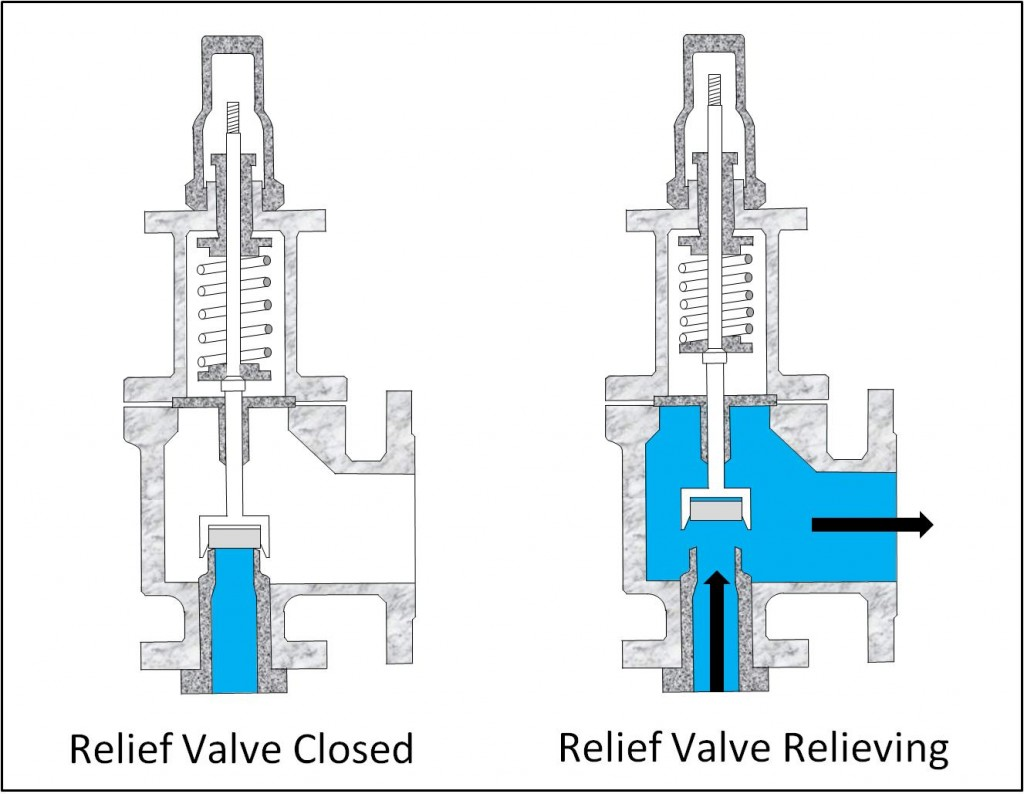
\includegraphics[scale=0.2]{media/safety-valve.jpg}
	\caption{Principe de fonctionnement d'une PSV.}
	\label{fig:safety-valve}
\end{figure}

\paragraph{Disque de rupture}
Un disque de rupture est aussi un dispositif
permettant de diminuer la pression en cas d'excès.
Il est constitué d'une membrane conçue pour céder
au-delà d'une certaine pression 
(voir figure \ref{fig:rupture-disc}). Un disque
de rupture est donc à usage unique (donc permet juste
d'évacuer la pression, pas de la réguler) et n'est pas
réglable (contrairement aux PSV) mais n'est pas
très cher et ne peut pas s'encrasser.

\begin{figure}[ht]
	\centering
	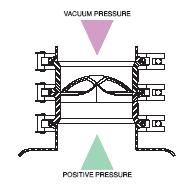
\includegraphics[scale=0.8]{media/rupture-disc.jpg}
	\caption{Principe de fonctionnement d'un disque de rupture.}
	\label{fig:rupture-disc}
\end{figure}

Comme dit précédemment, il est possible de combiner
PSV et disques de ruptures. Cela consiste à
placer un disque de rupture à l'entrée de la PSV
afin que celle-ci ne soit en contact avec les élements
chimiques que lorsque la pression est trop haute. Le
disque de rupture protège alors chimiquement le PDV et
limite la corrosion.

\subsection{Principe d'un échangeur de chaleur}
Un échangeur de chaleur est un dispositif permettant
de transférer de l'énergie thermique d'un fluide
vers un autre, sans les mélanger. Le flux thermique
traverse la surface d'échange qui sépare les fluides.
Le composant 124-MC rencontré dans la tâche 4 est un
échangeur de chaleur.

\subsection{Notions de sécurités industrielle}
\subsubsection{Gestion du risque}
\paragraph{Danger} Le terme danger désigne une situation
qui menace dans une certaine mesure la vie, l'environnement
ou la propriété.
Un concept clé pour l'identification des dangers est la
présence d'énergie ou de produit. Des dommages ou des dégats
peuvent avoir lieu s'il y a contact entre les produits
et une cible, ou s'il y a un transfert d'énergie vers une cible.
\paragraph{Risque} Le risque est un concept intellectuel qui
a été invenité pour rendre possible la discussion à propos
d'incertitude pour une situation particulière. On utilise
ce concept de risque pour communiquer à propos de la
possibilité qu'un danger puisse faire des dégâts.

Il y a plusieurs façon d'approcher le concept de risque :
\begin{itemize}
	\item Les approches pragmatique :
	\begin{itemize}
		\item Approche actuarielle ;
		\item Approche toxicologique et épidémiologique ;
		\item Approche de l'ingénieur (probabilité) ;
		\item Approche économique (comparaison risque et
		bénéfice).
	\end{itemize}
	\item Les approches multi-dimensionnelles :
	\begin{itemize}
		\item Approche psychologique ;
		\item Théories sociales ;
		\item Théories historiques et curlturelles.
	\end{itemize}
\end{itemize}

Dans le cadre des risques technologiques, les approches
multi-dimensionnelles sont difficiles à utiliser. On
utilise donc une approche pragmatique : l'approche
de l'ingénieur. Dans cette approche, on calcule le risque
comme suit :
\[ \text{Risque } = \text{ Probabilité} \times \text{ Dégâts}. \]
On peut donc calculer, mesurer, comparer, comprendre les
risques.

\section{Connaissance du procédé de synthèse de l'ammoniac}
On peut résumer la chimie industrielle de l'azote comme suit :
\begin{chemmath}
	N_2 \rightarrow NH_3 \rightarrow HNO_3 \rightarrow NH_4NO_3
	\rightarrow \text{engrais}.
\end{chemmath}
Notons qu'on peut également utiliser le \chemform{NH_3} et le \chemform{HNO_3}
pour produire des matières plastiques (fibres acryliques, polyamides)
et pour produire des insecticides, des fondigicides\footnote{Un fongicide
est une substance conçue exclusivement pour éliminer ou limiter le
développement des champignons parasites des végétaux.}, etc.

\subsection{Etapes principales du procédé (tel que schématisé dans la tâche 1)}
Pour situer les différents blocs dans le procédé général, voir 
flow-sheet à la figure \ref{fig:flow-sheet}.
\subsubsection{Généralités}
Pour produire l'ammoniac, on utilise le procédé Haber-Bosch
dont la réaction s'écrit
\begin{chemmath}
	N_2 + 3H_2 \rightarrow 2NH_3.
\end{chemmath}
Un catalyseur est aussi souvent utilisé.
Les conditions opératoires sont une température
aux alentours des \unit{500}{\degreecelsius} et
une pression de 100 à 1000 bars.

Cette réaction a besoin de deux matières
premières :
\begin{itemize}
	\item \chemform{N_2} : que l'on prend dans l'air
	directement ;
	\item \chemform{H_2} que l'on peut se procurer
	de plusieurs manières :
	\begin{itemize}
		\item Carbochimie ;
		\item Pétrochimie ;
		\item Gaz naturel.
	\end{itemize}
\end{itemize}

\subsubsection{Fabrication du gaz de synthèse}
Pour fabriquer le gaz de synthèse \chemform{H_2}
dont nous avons besoin, on utilise le gaz naturel
\chemform{CH_4} dans une réaction que l'on appelle
le reforming primaire 
\begin{chemmath}
	CH_4 + H_2O \Leftrightarrow CO + 3H_2 \text{ (endothermique)}.
\end{chemmath}
Il y a également plusieurs réactions secondaires à
considérer, dans le cadre du projet, on ne considère
que la suivante
\begin{chemmath}
	CO + H2_O \Leftrightarrow CO_2 + H_2.
\end{chemmath}
Les conditions opératoires sont une pression
de \unit{25-30}{\bbar} et une température
de réaction de \unit{750-800}{\degreecelsius}.
On utilise souvent des anneaux de nickel comme
catalyseur.
On note aussi que cette réaction est largement
endothermique et a donc besoin d'énergie pour avoir
lieu.

\subsubsection{Apport d'énergie au reforming primaire : le four}
La réaction du reforming primaire a besoin
d'énergie pour avoir lieu, cette énergie est apportée
par le four. Dans le cadre du projet, la réaction
du four est
\begin{chemmath}
	CH_4 + 2O_2 \rightarrow CO_2 + H_2O \text{ (exothermique)}.
\end{chemmath}
On considère que le four a un rendement de 75\%.

\subsubsection{Reforming secondaire oxydant}
La réaction du reforming secondaire est
\begin{chemmath}
	CH_4 + \frac{1}{2}O_2 \rightarrow CO + 2H_2.
\end{chemmath}
Cette réaction permet de retirer le \chemform{CH_4} qui n'a
pas réagit dans le reforming primaire. % FIX : quelque confirme ça?
Des réactions secondaires ont également lieu mais elles
sont négligées dans le cadre du projet.
Les conditions opératoires sont une pression
de \unit{25-30}{\bbar} et une température
de \unit{900}{\degreecelsius} de telle sorte
qu'une combustion partielle ait lieue.
On utilise souvent le nickel comme catalyseur.

\subsubsection{Conversion du \chemform{CO} : Water-Gaz-Shift}
Dans le bloc du Water-Gaz-Shift, on a la réaction
suivante
\begin{chemmath}
	CO + H_2O \Leftrightarrow CO_2 + H_2 \text{ (exothermique)}. 
\end{chemmath}
Le facteur limitant de cette réaction est la température.
En diminuant la température, l'équilibre est avantageusement
déplacé mais la cinétique est fortement ralentie. On
utilise donc habituellement un convertisseur à deux étages :
\begin{itemize}
	\item	Etage 1 : la température est aux alentours de
	\unit{400}{\degreecelsius} de telle sorte que la cinétique
	ne soit pas trop ralentie. On peut alors utiliser
	des catalyseurs bon marché. 70\% à 80\% de la conversion a lieu
	ici ;
	\item Etage 2 : la température est aux alentours de
	\unit{200}{\degreecelsius}, c'est pourquoi il faut utilise
	des catalyseurs plus chers pour accélerer la réaction.
\end{itemize}

Néanmoins ces aspects du Water-Gaz-Shift n'ont pas
vraiment été abordé dans le cadre du projet.

\subsubsection{Décarbonatation}
Le principe est d'absorber ou de récupérer le \chemform{CO_2}.

\begin{figure}[ht!]
	\centering
	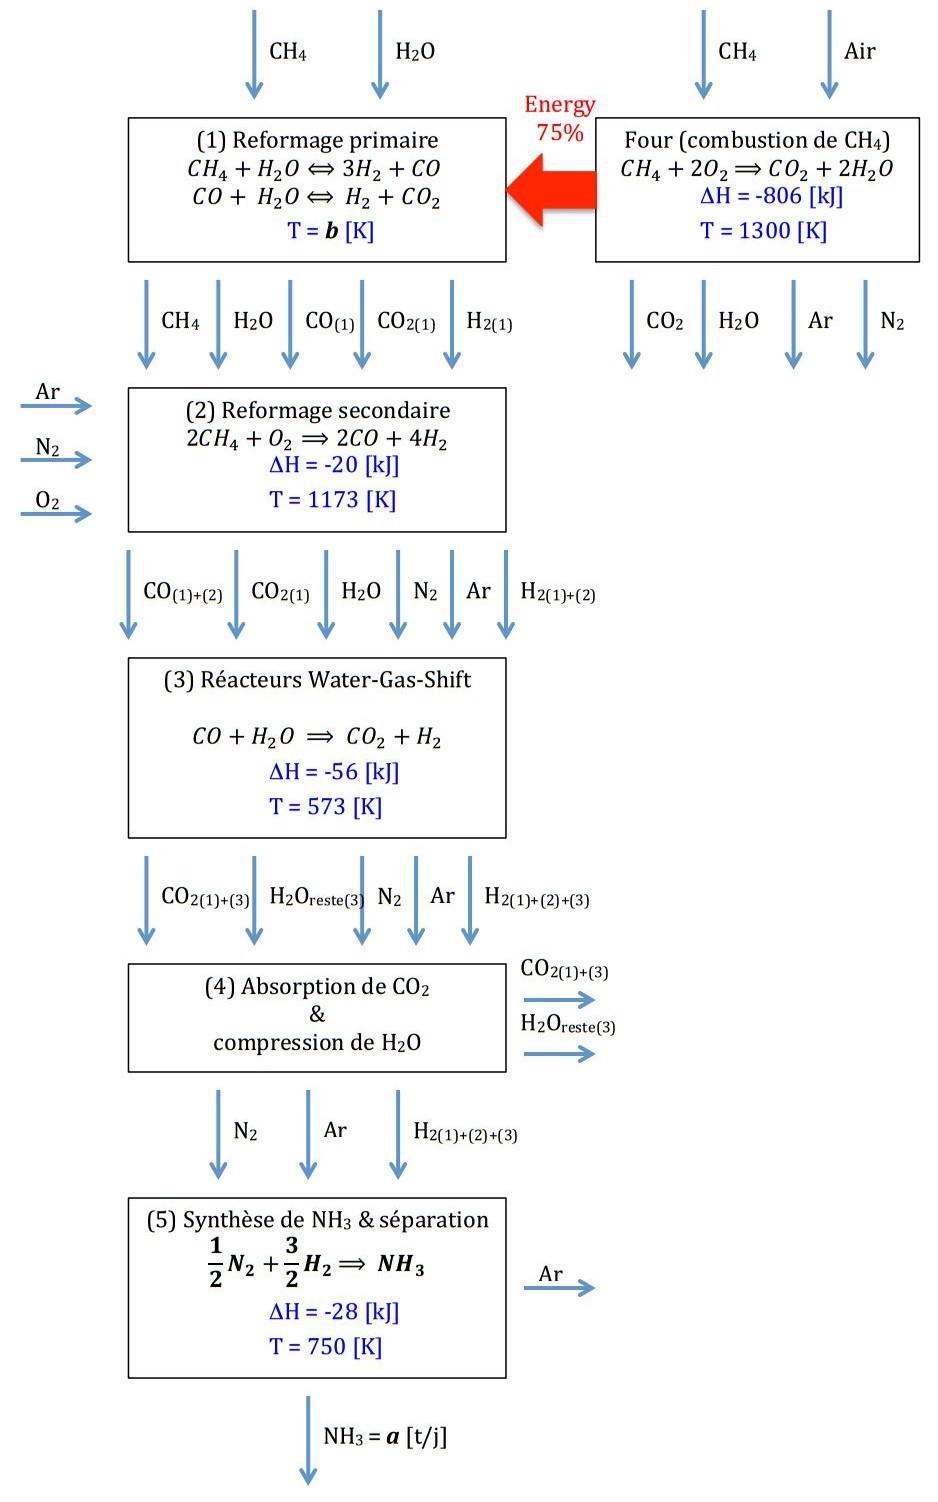
\includegraphics[scale=0.6]{media/flow-sheet-v2.jpg}
	\caption{Flow-sheet.}
	\label{fig:flow-sheet}
\end{figure}

\subsection{Fonctionnement du réacteur de synthèse}
Le réacteur de synthèse se compose des élements suivants 
(voir figure \ref{fig:flow-sheet-aspen}) :
\begin{itemize}
	\item Un compresseur isentropique ;
	\item Un préchauffeur ;
	\item Un réacteur ;
	\item Un refroidisseur ;
	\item Une unité flash pour la séparation des produits ;
	\item Un spliter pour la purge.
\end{itemize}
Les différentes conditions opératoires sont reprises
sur la figure \ref{fig:flow-sheet-aspen}.
\begin{figure}[ht!]
	\centering
	\rotatebox{90}{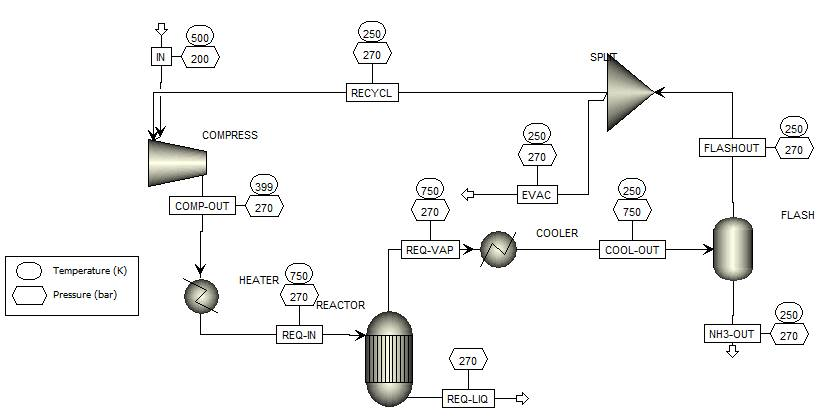
\includegraphics[scale=0.5]{media/flow-sheet-aspen.jpg}}
	\caption{Flow-sheet du réacteur de synthèse.}
	\label{fig:flow-sheet-aspen}
\end{figure}

\subsection{Principe du recyclage de réactifs et de la purge}
La réaction de synthèse d'ammoniac se passe à l'équilibre thermodynamique.
On travaille à pression constante puisque nous sommes en système ouvert. 
Le but du recyclage est de maximiser le rendement seulement on se rend 
compte que il  va y avoir une accumulation d'argon dans le réacteur si 
l'on renvoie à l'entrée de celuui-ci, la totalité de ce qui n'a pas réagit. 
Il est donc nécessaire de faire une purge, c'est-à-dire rejeter un certain 
coefficient de \ce{N2}, de \ce{H2} et de \ce{Ar}. Pour le calcul de la constante
d'équilibre, on procède exactement de la même manière que pour le réformage primaire. 
On avait l'expression suivante : 
$$K(T) = \frac{4x\cdot p\std \cdot n_{g,tot}}{(2n_1 - x)^{1/2} (2n_2 - 3x)^{3/2} \cdot p_{tot}}.$$
Il est important de comprendre que $n_1, n_2 et n_3$ représentent l'ensemble
de ce qui rentre respectivement en \ce{N2, H2 et Ar}, c'est-à-dire les recyclages compris.
Ensuite, nous posons un coefficient $k$ de proportion qui est le rapport
entre ce qui est recyclé et ce qui sort du réacteur. On peut faire l'hypothèse
que la purge enlève une proportion égale de moles pour chaque composé. Cela 
signifie que le rapport $k$ est le même pour les 3 composés. Nous l'avions 
choisi : $k \in [0 \text{(ouvert)}, 1 \text{(fermé)}[$.
Enfin, la dernière chose importante à  faire est de s'assurer qu'il n'y ait pas
d'accumulation d'argon dans le réacteur ce qui entrainerait une baisse de rendement. 
Il faut donc que en régime, l'argon rentrant soit égal à l'argon purgé. On a alors : 
$\ce{Ar_{syn}} = \ce{Ar_{in}+Ar_{rec}}$. 
Finalement, si l'on veut pouvoir exprimer les entrées en fonction du rapport de 
purge, de la pression, la température et le débit d'ammoniac sortant on doit se 
mettre dans la condition idéale ou les débits sont parfaitement conformes aux
coefficients stœchiométriques.

\subsection{Points principaux de production et de consommation d'énergie du procédé}
Le réformeur primaire est le plus gros consommateur d'énergie, c'est d'ailleurs
la seule réaction endothermique du procédé. L'énergie requise est apportée par
le four, qui a un rendement de 75\%.

\subsection{Principaux risques pour la santé et l'environnement liés aux réactifs et produits}
\paragraph{Le méthane} Le méthane est un gaz à effet de serre qui influe
sur le climat. Il est considéré comme le 3ème gaz responsable du
réchauffement climatique.
\paragraph{Le monoxyde de carbone} Il peut causer des intoxications s'il est
présent trop importante. Sur le long terme, il augmente le risque de maladie
cardiovasculaire. Le \chemform{CO} est également impliqué de façon majeure
dans les effets de la pollution atmosphérique.
\paragraph{Diazote} A priori aucun effet nocif pour l'environnement.
\paragraph{Argon} Risque de suffocation dans les secteurs confinés, peut
entrainer des vertiges, nausées, vomissements, pertes de consience et la mort.
L'argon ne présente aucun risques connus pour l'environnement.
\paragraph{Dioxyde de carbone} Le \chemform{CO_2} serait le deuxième
gaz à effet de serre le plus important dans l'atmosphère après la vapeur
d'eau, contribuant à hauteur de 26\% et 60\% à ce phénomème. Ce gaz
est également dangereux pour la santé et peut même être mortel si
la concentration dans l'air est trop élevée.
\paragraph{Dihydrogène} Dangeureux si à inhalation, peut être mortel.
Aucun effet sur l'environnement, le gaz
sera rapidement absorbé dans des secteurs bien-aérés. Aucun
effet non plus sur les animaux ou la vie aquatique connus à l'heure
actuelle.
\paragraph{Ammoniac} C'est un des principaux responsables
de l'acidification des sols et des bois. L'ammoniac rejeté
dans l'atmosphère favorise aussi les pluies acides. Il 
n'intervient cependant pas dans le réchauffement climatique et n'a pas
d'effet sur la couche d'ozone. L'ammoniac
est également nuisible pour les mieux aquatiques et certains
animaux primitifs. Enfin, la production d'ammoniac est une grande
consommatrice d'électricté, représentant jusqu'à 2\% de la
production mondiale.

L'ammoniac est également toxique pour l'être humain et a
diverses conséquences sur la santé.
\paragraph{Oxydes d'azote} Les oxydes d'azotes \chemform{NO_x}
représentent le \chemform{NO} et \chemform{NO_2}, ce sont
deux polluants atmosphériques. Le \chemform{NO_2} est aussi
un gaz à effet de serre. Ils interviennent également
dans les pluies acides.
Le \chemform{NO_2} est très toxique (40 fois plus que le
\chemform{CO} et 4 fois plus que \chemform{NO}) et
pénètre profondément dans les poumons.

\section{Laboratoire d'électrolyse de l'eau}

\section{Questions de réflexion sur les thématiques traitées
dans le cadre du projet}
\subsection{Compréhension globale des impacts du procédé de l'ammoniac sur l'environnement}
Le processus utilisé est extrément polluant en terme de rejet de \chemform{CO_2}, et
plus particulièrement le Water-Gas-Shift et le réformeur primaire.
\subsection{Compréhension globale des stratégies mises en place pour limiter la consommation 
énergétique sur un site de production d'ammoniac tel celui de Yara}

\end{document}